\chapter{The First Analog Prototype: First Resets and Leakage Measurements}~\label{chap:saq}

In this chapter we present the first implementation of the Q-Pix front-end design using off-the-shelf electronics.

This section describes the first prototype based on the Q-Pix readout: The Simplified Analog Q-Pix (SAQ).
First we discuss the design goals of the prototype and highlight the basic building blocks of any Q-Pix based prototype.
Next, We describe the prototype status as well as lessons learned in characterizing noise and performing calibrations.

In the final part of this section we describe the future goals of this prototype, including the calibration of the detector response with Gas Electron Multipliers (GEMs)~\citep{SAULI20162} and promising future analysis.
We emphasize that at the time of the writing of this thesis the results of this experiment are incomplete.
Nevertheless, the lessons learned so far, particularly in the calibration procedure, are useful to explore the abilities of the Q-Pix readout.
The final results of SAQ are just beyond the scope of this work, but I provide SAQ's details here as a means of introducing the front-end of Q-Pix as well as highlighting my personal contributions to Q-Pix's overall development.

The entire data acquisition (DAQ) chain used for both SAQ experimental setups are my sole independent work.
My contributions include the the development and deployement firmware on the Zybo-Z7 FPGA, as well as the embedded software code on the integrated SoC processing system.
I developed the the Python3 software which handles packet communication as well as the GUI for data collection.
I also developed the data storage trees, which are the original containers for all data used in the analysis. 
Additionally, I wrote analysis scripts used for the work done at the SAQ site at the University of Texas at Arlington.

\section{Simplified Analog Q-Pix: System Design}

\begin{figure}[]
\centering
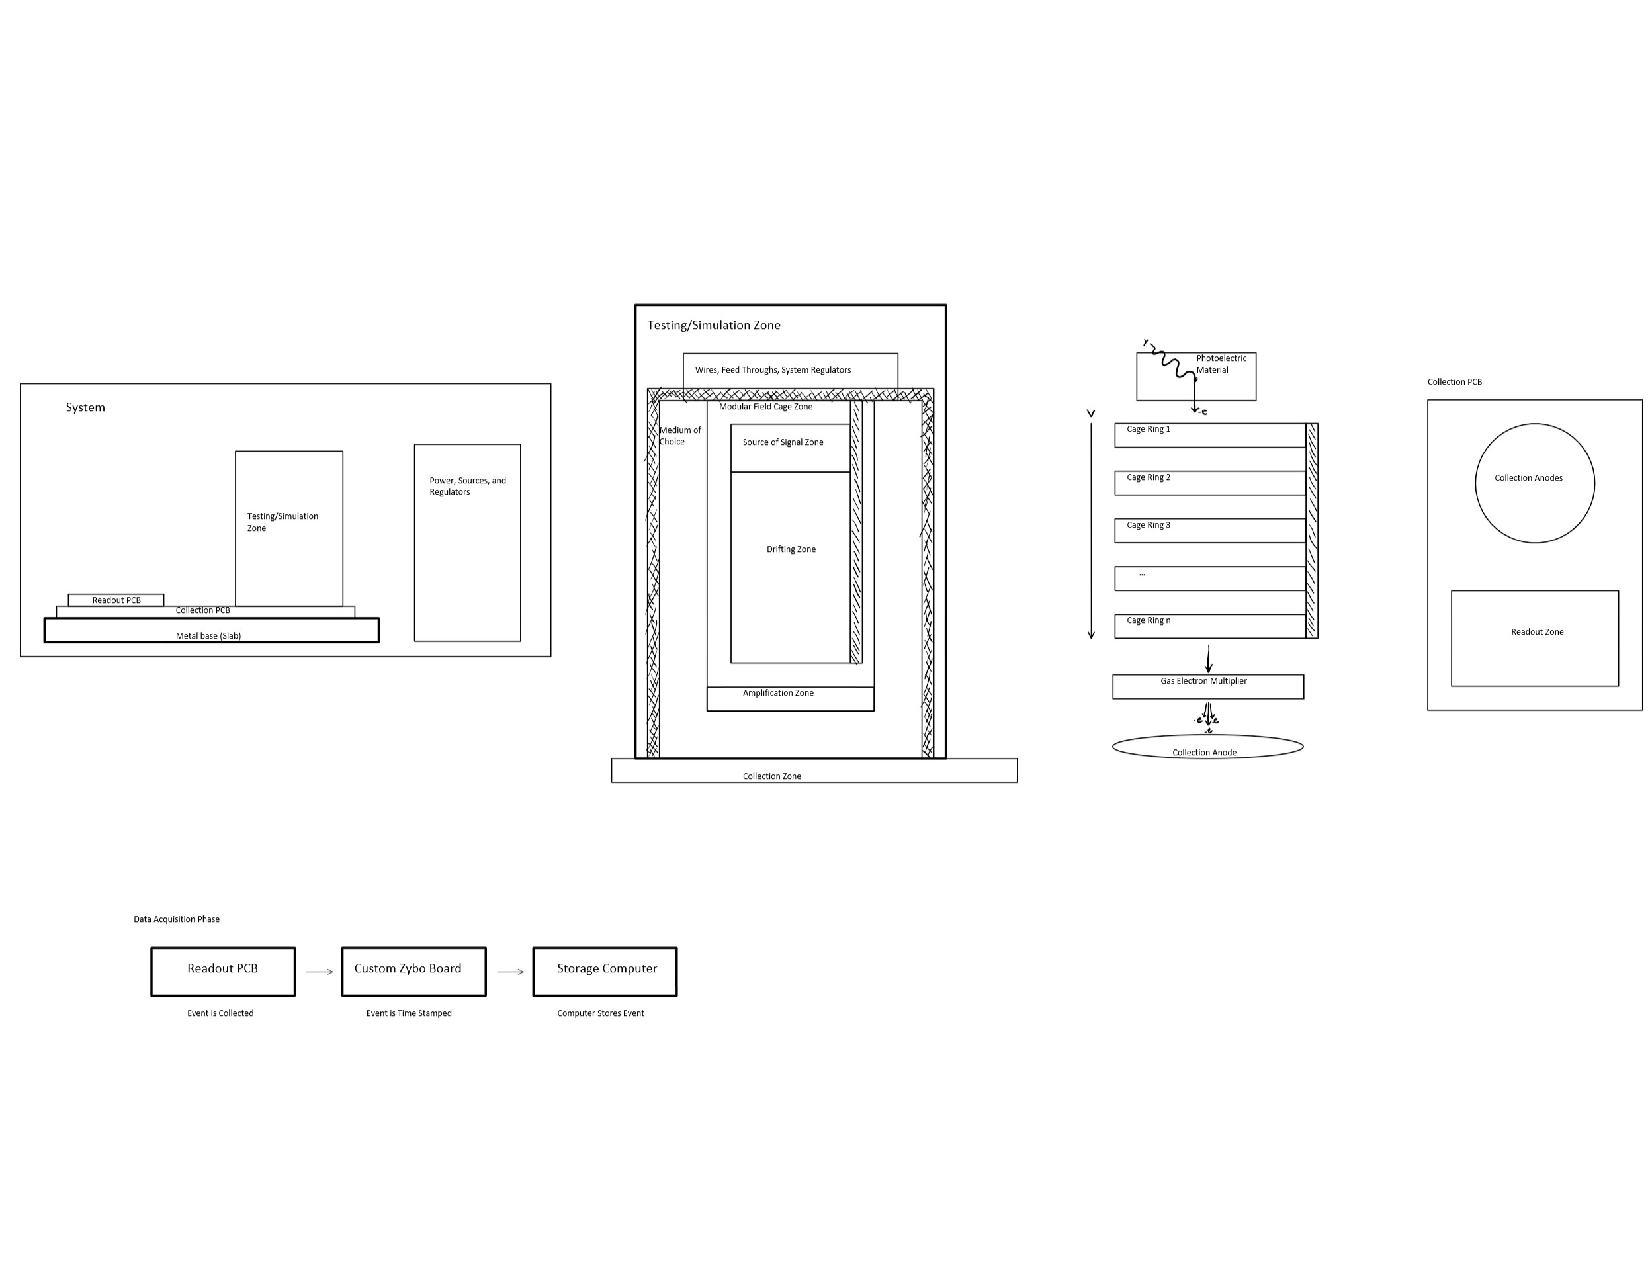
\includegraphics[width=\textwidth]{images/SAQ_setup_diagram.pdf}
\caption{The SAQ Setup model based on~\ref{fig:saq_setup_flatten}.}
\label{fig:saq_physical_setup_flatten}
\end{figure}


\begin{figure}[]
\centering
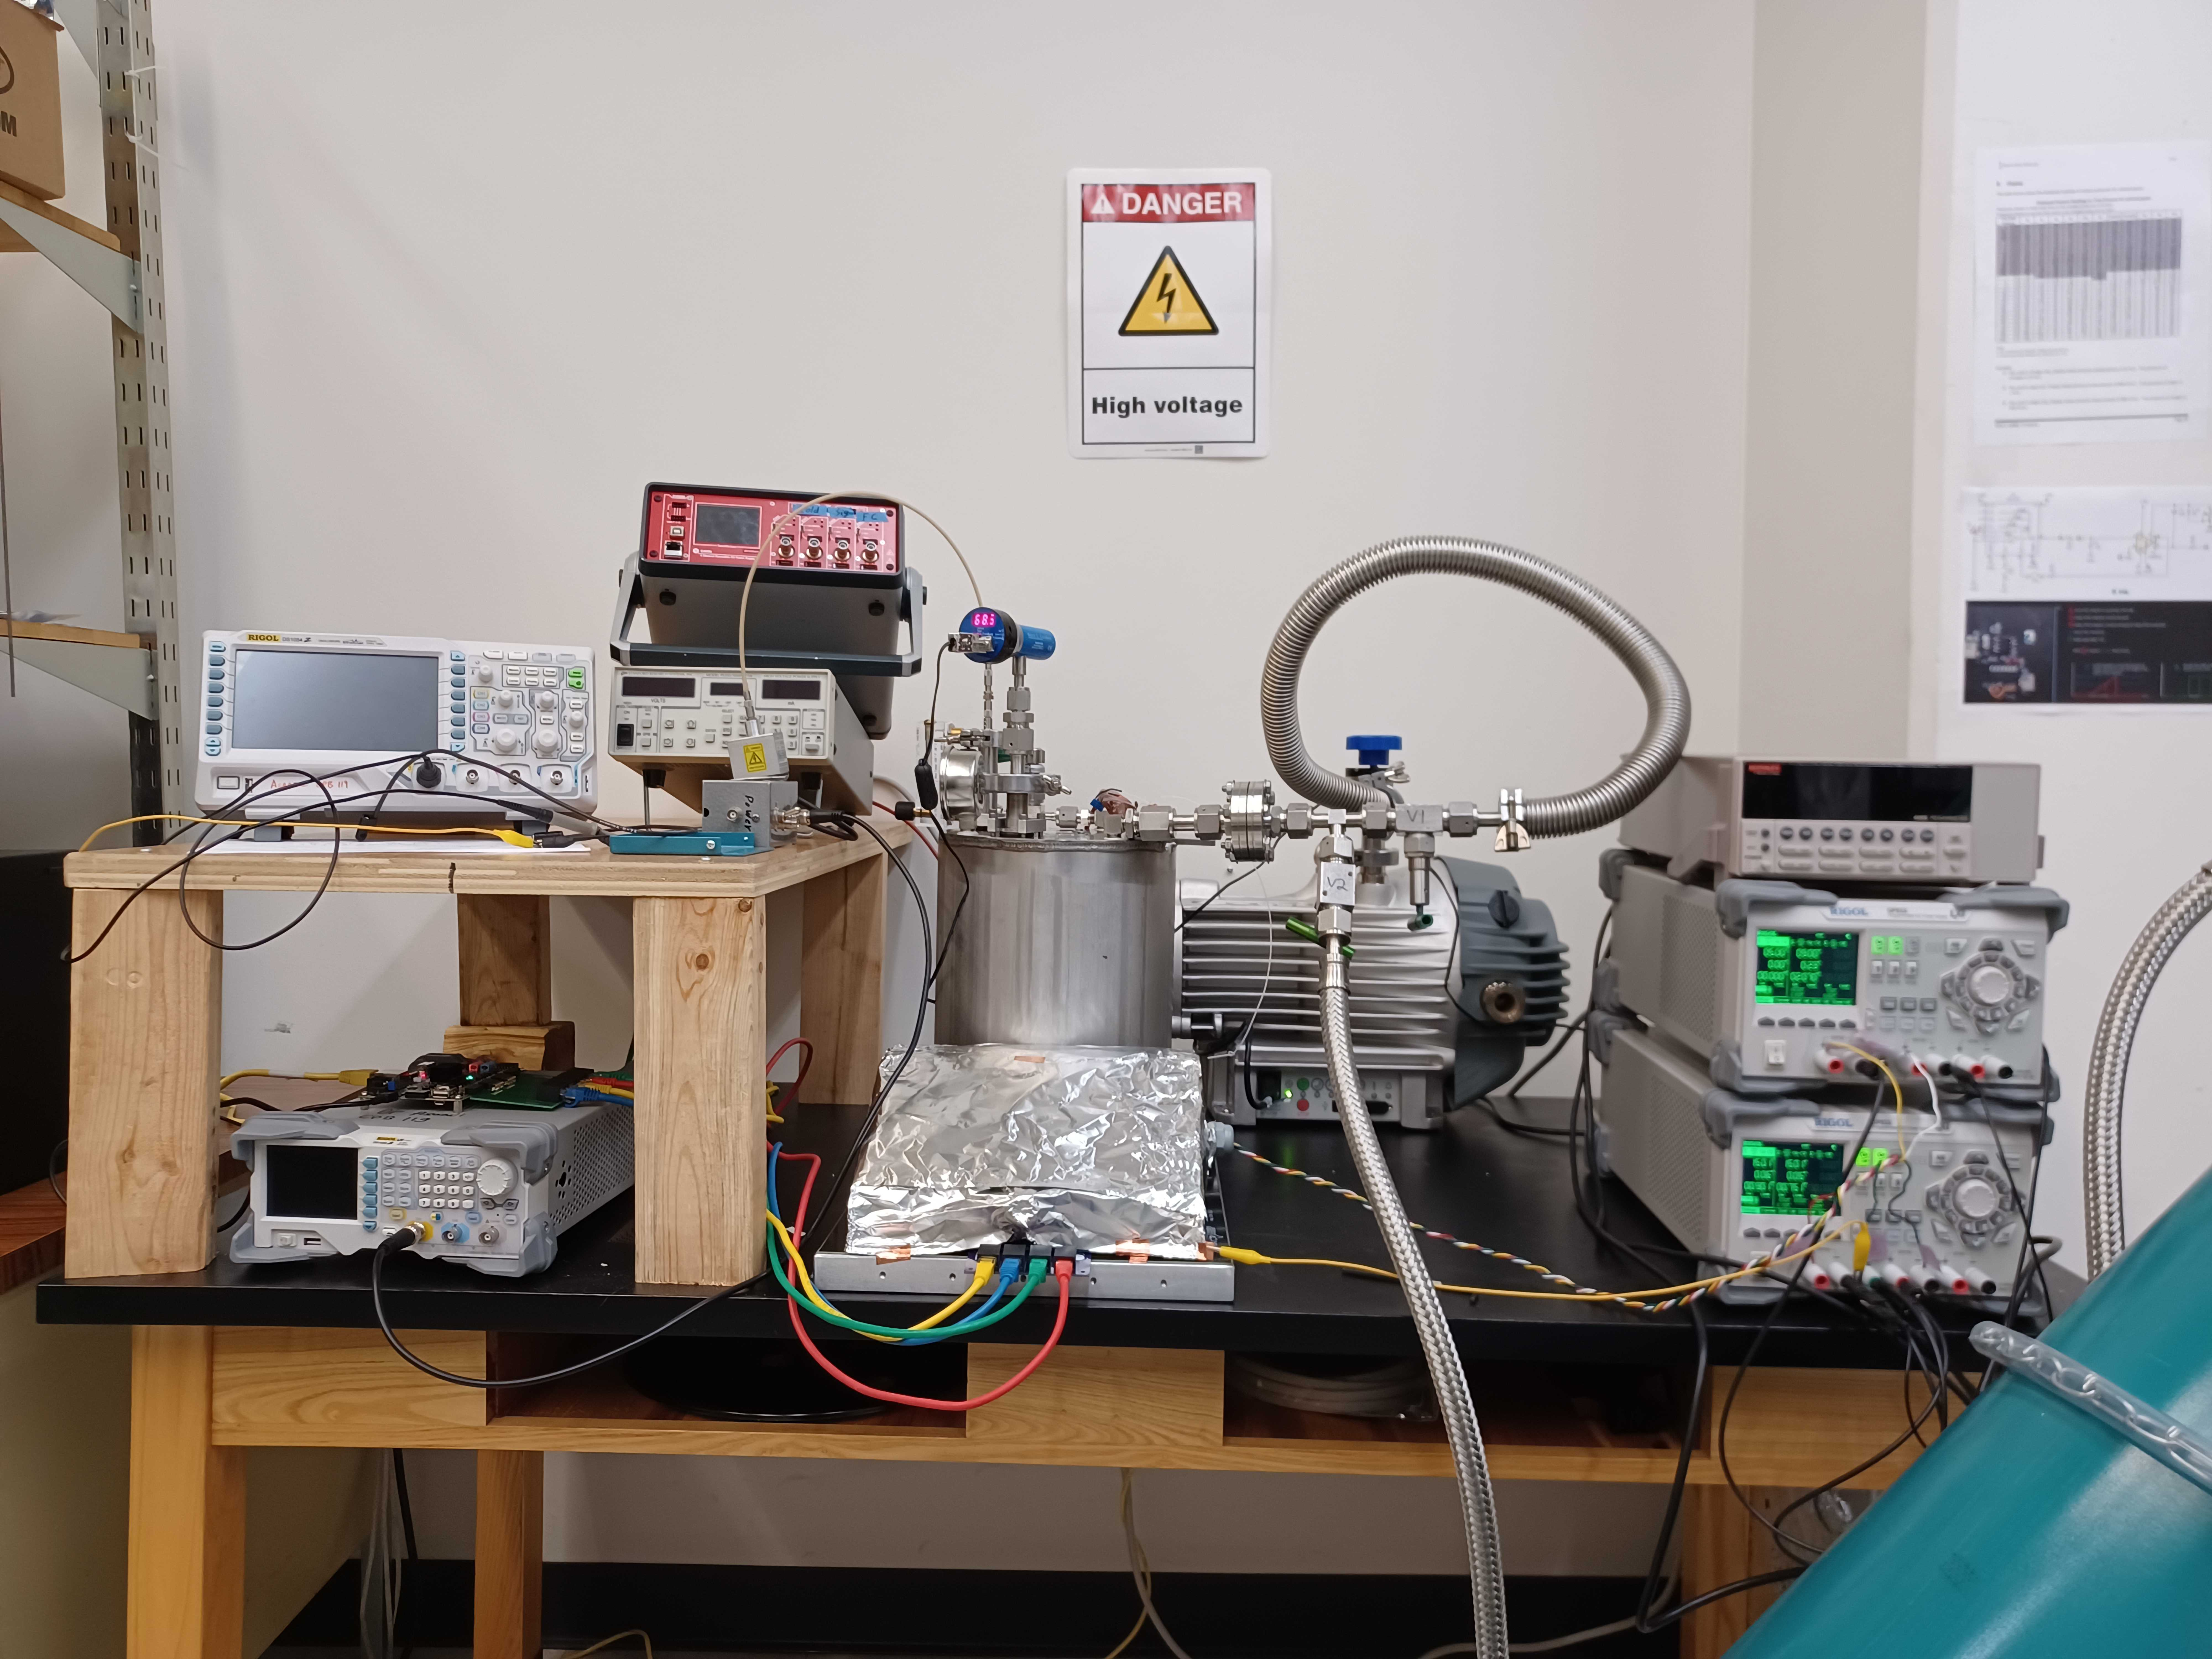
\includegraphics[width=\textwidth]{images/SAQ_physical_setup.jpg}
\caption{The SAQ setup at UTA.
In the center is the TPC, SAQ board~(Figure~\ref{fig:saq_readout_board}), and pump as shown in Figure~\ref{fig:saq_physical_setup_flatten}.
}
\label{fig:saq_setup_flatten}
\end{figure}


\begin{figure}[]
\centering
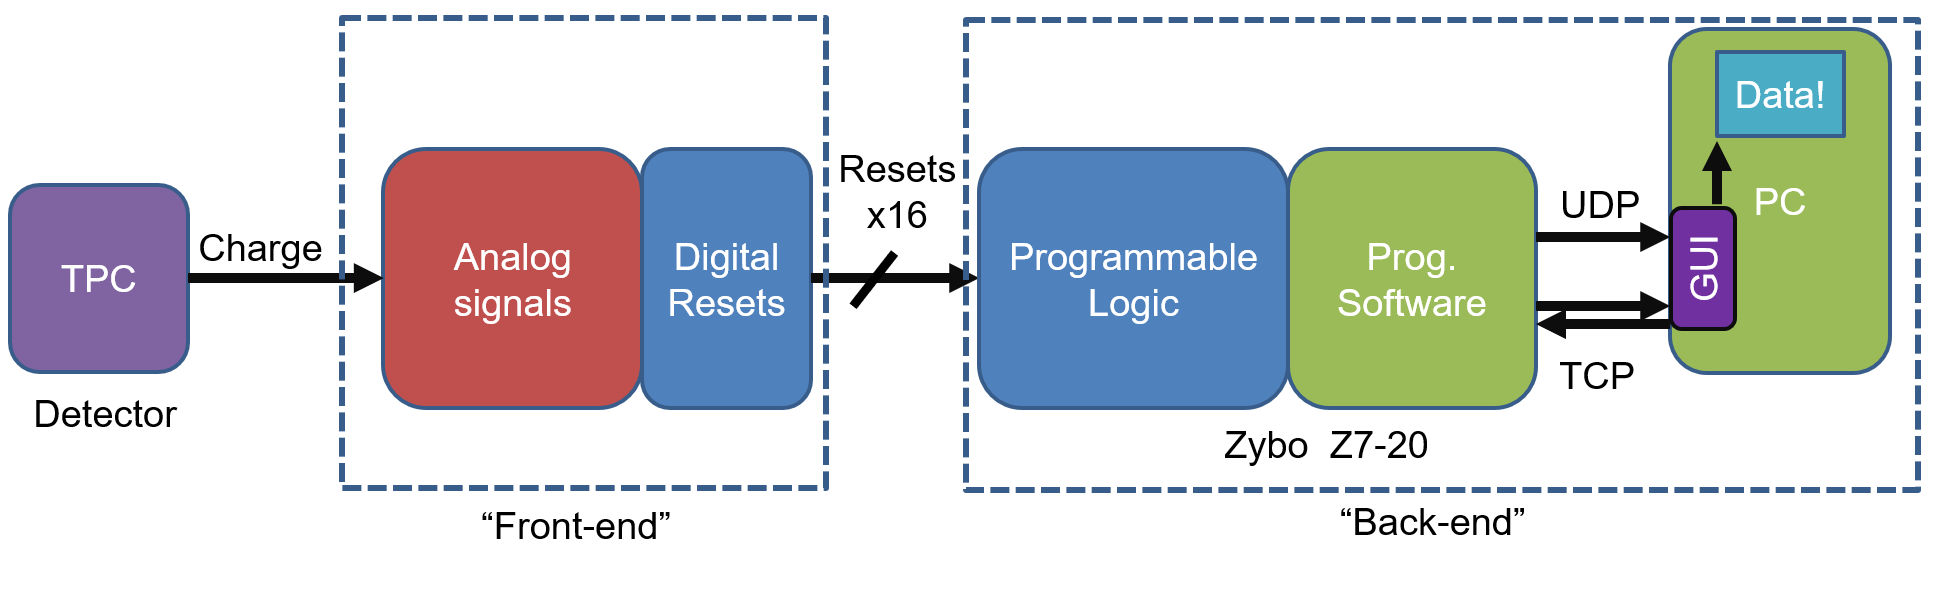
\includegraphics[width=\textwidth]{images/saq_daq_back-end_summary.png}
\caption{SAQ System over view connecting the front-end and back-end parts of a Q-Pix readout.
Gaseous Argon is used for the drift medium of the TPCs at both UTA and Wellesley.
Accumulated charge is read by the front-end which consists of 16 integrating amplifiers each connected to a comparator used as a trigger~\ref{fig:saq_circuit_kicad}.
The back-end consists of a single prototype board, the Zybo-Z7~(Figure~\ref{fig:saq_zybo}).
}
\label{fig:saq_diagram}
\end{figure}


\subsection{The TPC Design}

%%
\begin{figure}[]
\centering
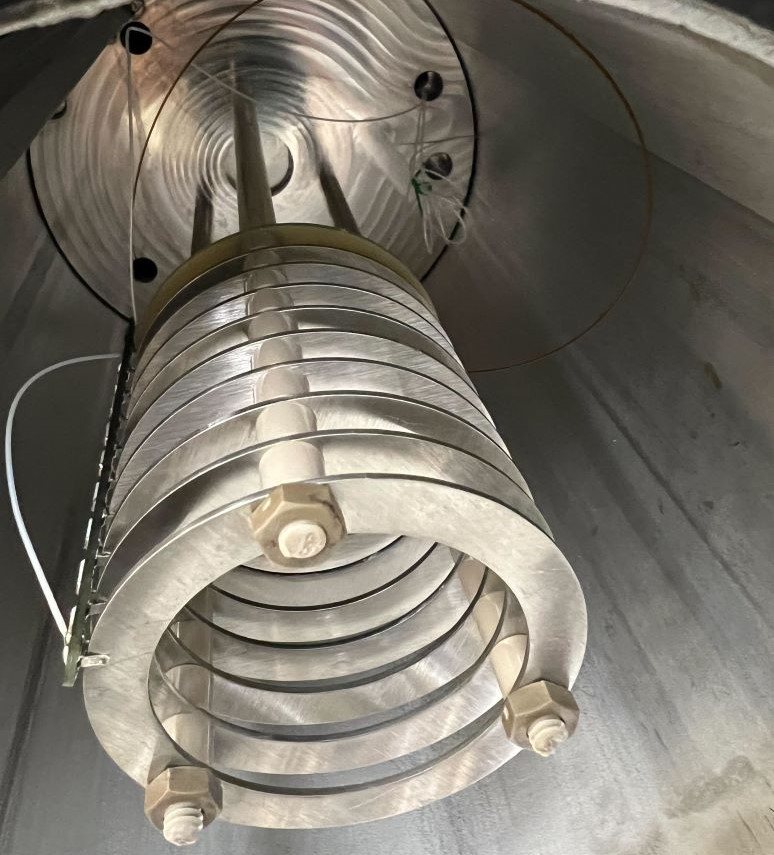
\includegraphics[width=\textwidth]{images/saq_fieldcase_rings.jpg}
\caption{}
\label{fig:saq_field_case}
\end{figure}


An image of the experimental setup performed at Wellesley University is shown in Figure~\ref{fig:wellesley_tpc}.

\begin{figure}[]
\centering
\begin{subfigure}{.5\textwidth}
  \centering
  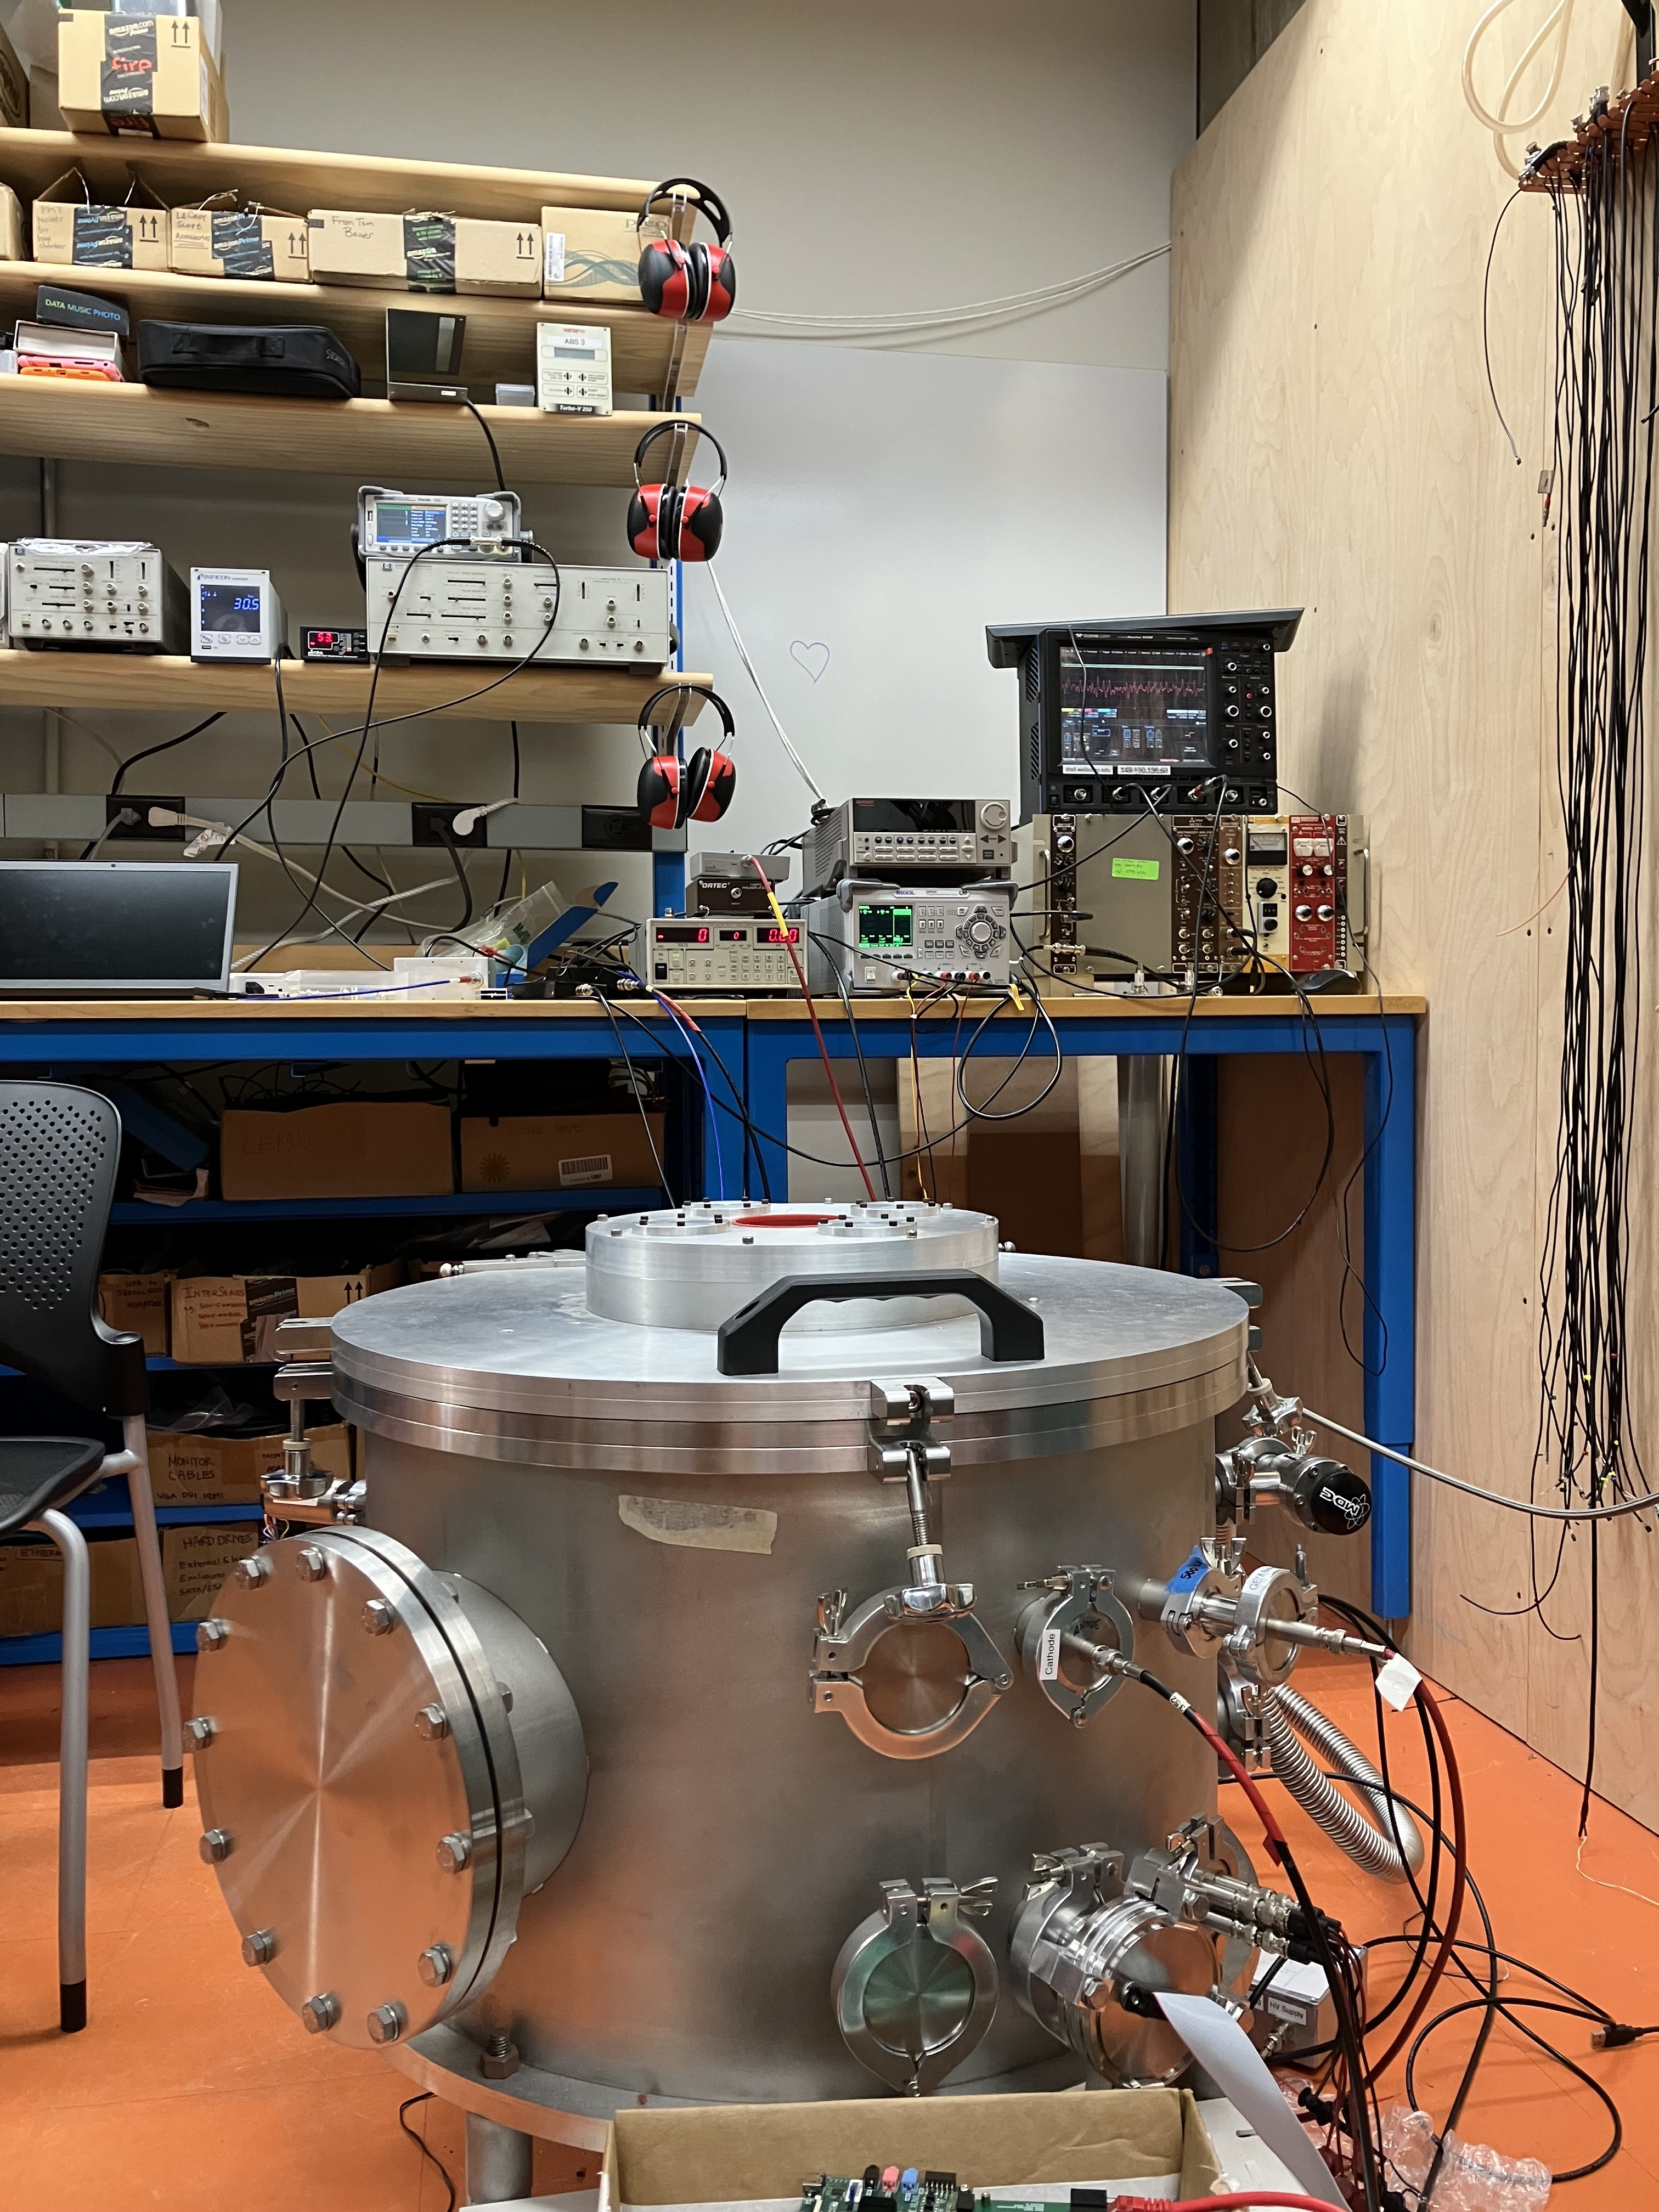
\includegraphics[width=\textwidth]{images/saq_wellesley_tpc.jpg}
  \caption{}
\end{subfigure}%
\begin{subfigure}{.5\textwidth}
  \centering
  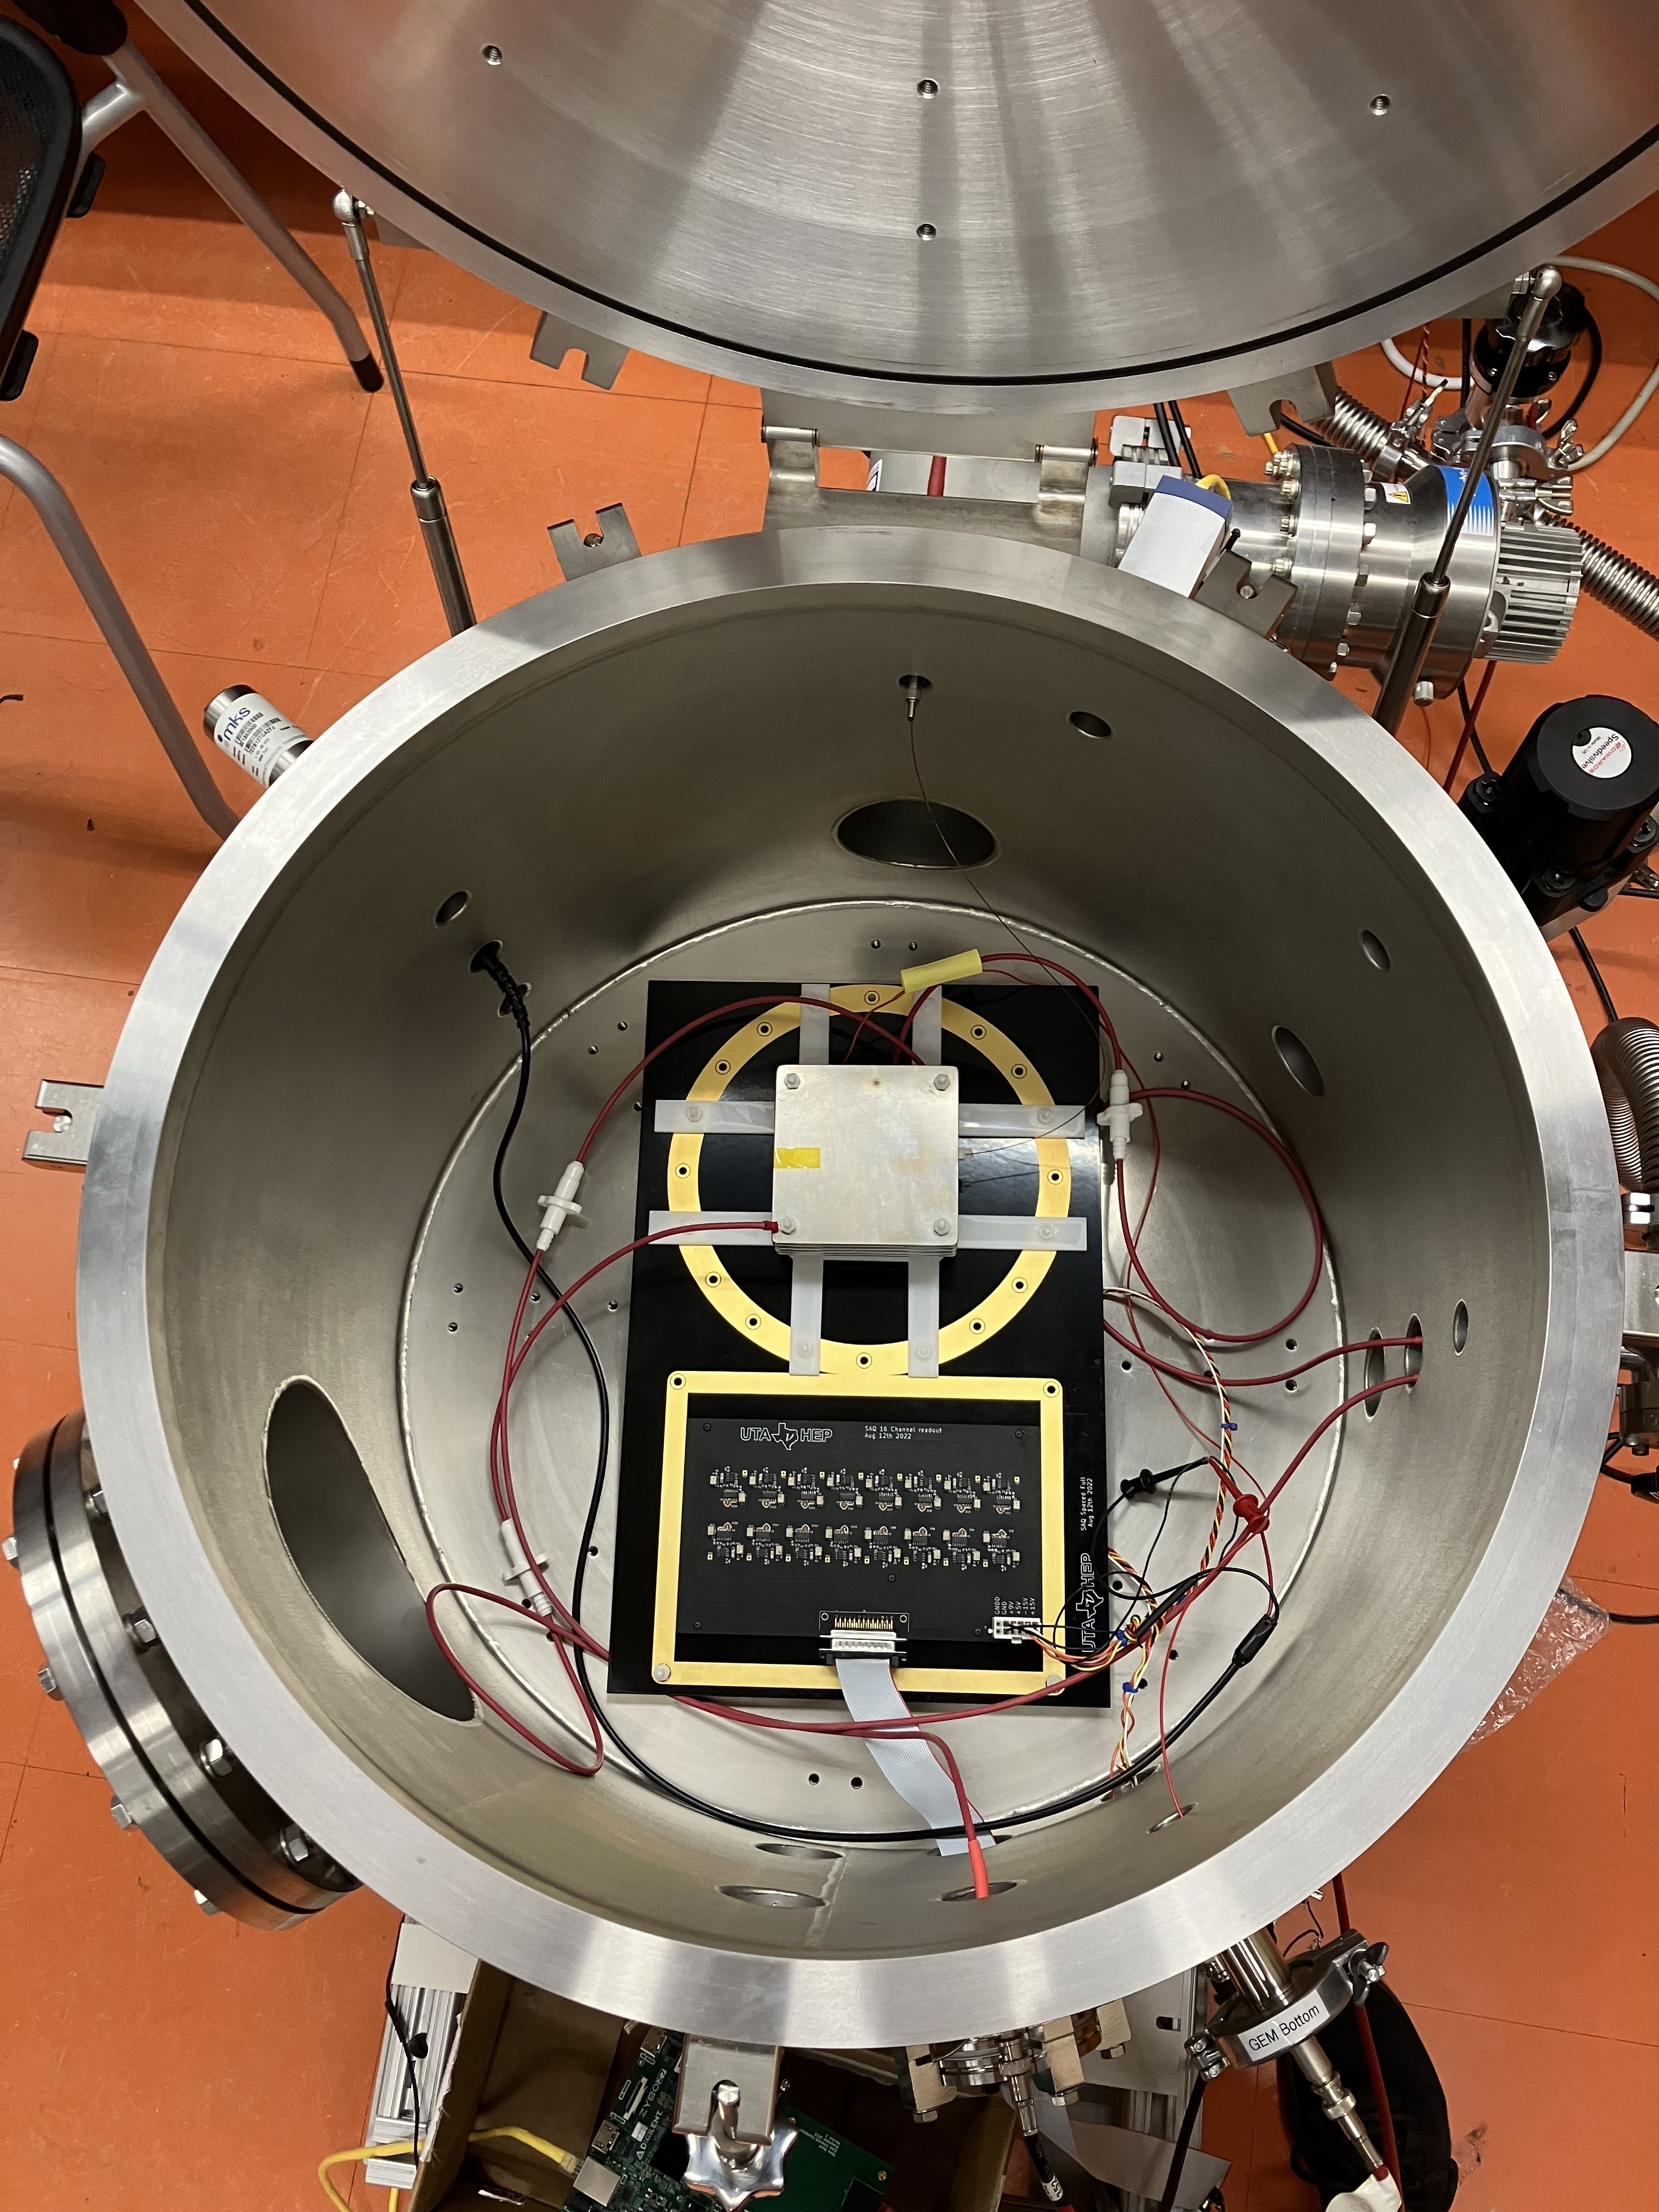
\includegraphics[width=\textwidth]{images/saq_wellesley_tpc_daq.jpg}
  \caption{}
\end{subfigure}
\caption{Picture of the TPC and DAQ setups at Wellesley University.}
\label{fig:wellesley_tpc}
\end{figure}

The GEM used is based on work presented in Ref.~\citep{THORPE2023167438}.

\begin{figure}[]
\centering
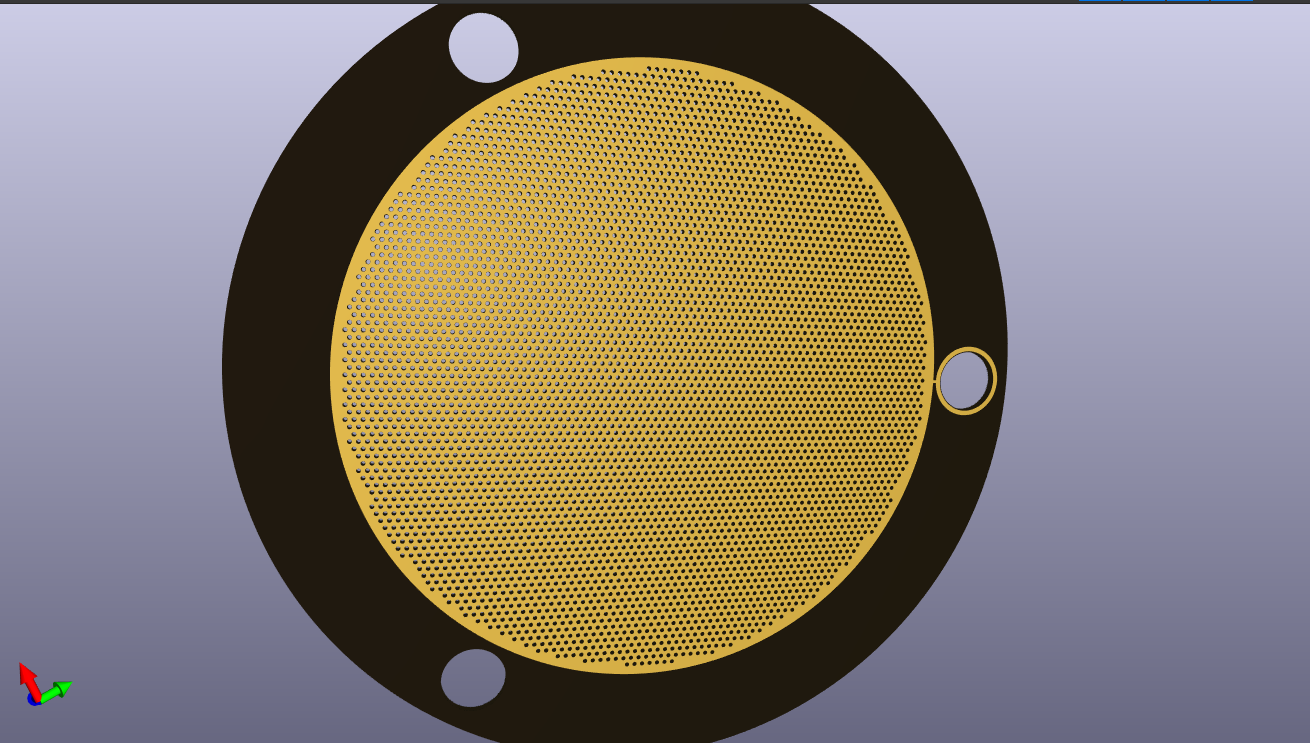
\includegraphics[width=0.5\textwidth]{images/ThGem_layout.png}
\caption{}
\label{fig:saq_th_gem_layout}
\end{figure}


\subsection{The Integrator Circuit}

The integrator circuit used in the SAQ experiment is shown in Figure~\ref{fig:saq_circuit_kicad}.
The Integrated Circuit (IC) used is the IVC-102~\citep{ivc_datasheet}, where the selected capacitor is 10~\unit{pF}.
We selected the lowest available capacitance of the IVC chip in order to ensure that resets are produced with the lowest amount of possible charge~\ref{eq:capacitor}.
Further configuration of the charge required per reset uses a configurable voltage (VDD in Figure~\ref{fig:saq_circuit_kicad}) with a variable resistor.
Charge is accumulated from the TPC as an input into the IVC chip.
The comparator sends an output pulse with a width of $\approx 10~\unit{\mu s}$ once the voltage on the IVC exceeds four times the voltage across VDD, due to the voltage divider.

\begin{figure}[]
\centering
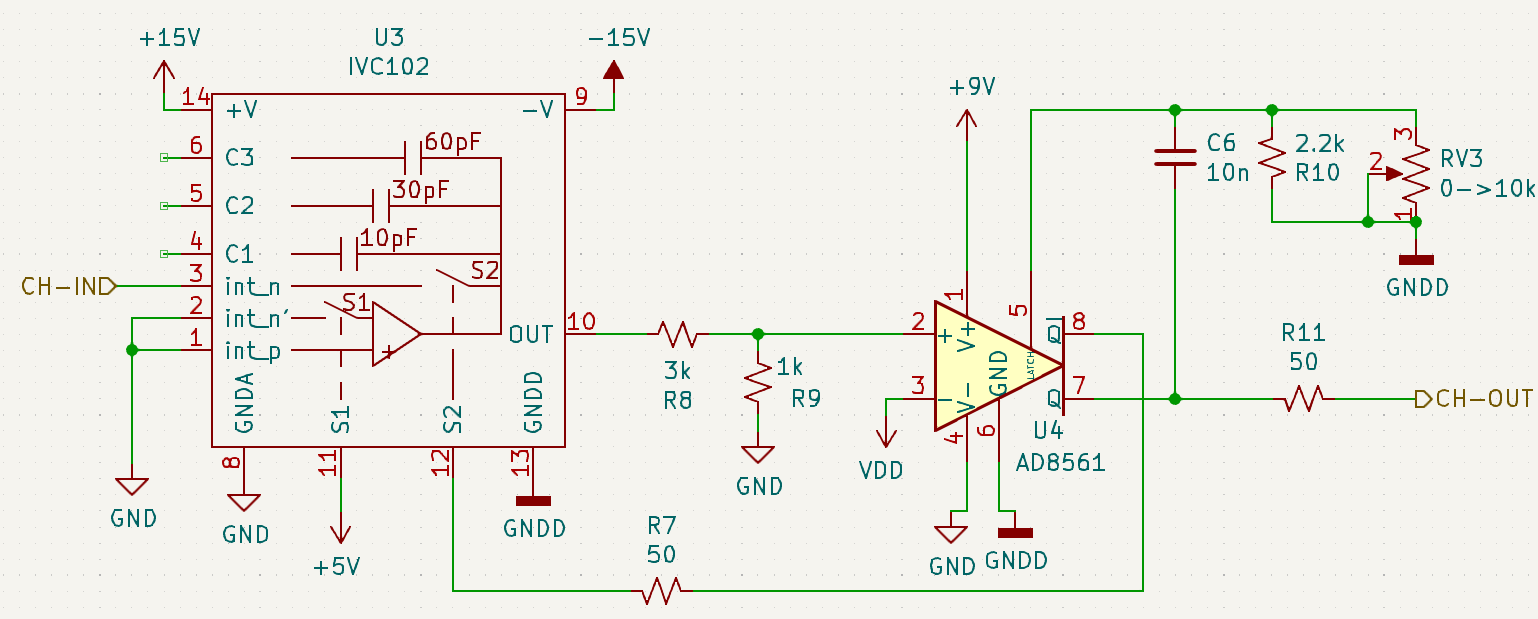
\includegraphics[width=\textwidth]{images/saq_integrator_circuit.png}
\caption{
A schematic of the front-end CSA and trigger components.
The IVC~\citep{ivc_datasheet} chip chosen as the off-the-shelf integrator for this experiment.
The main selection choice for this part is due to its low input bias current $\ll 750~\unit{fA}$.
}
\label{fig:saq_circuit_kicad}
\end{figure}

\begin{figure}[]
\centering
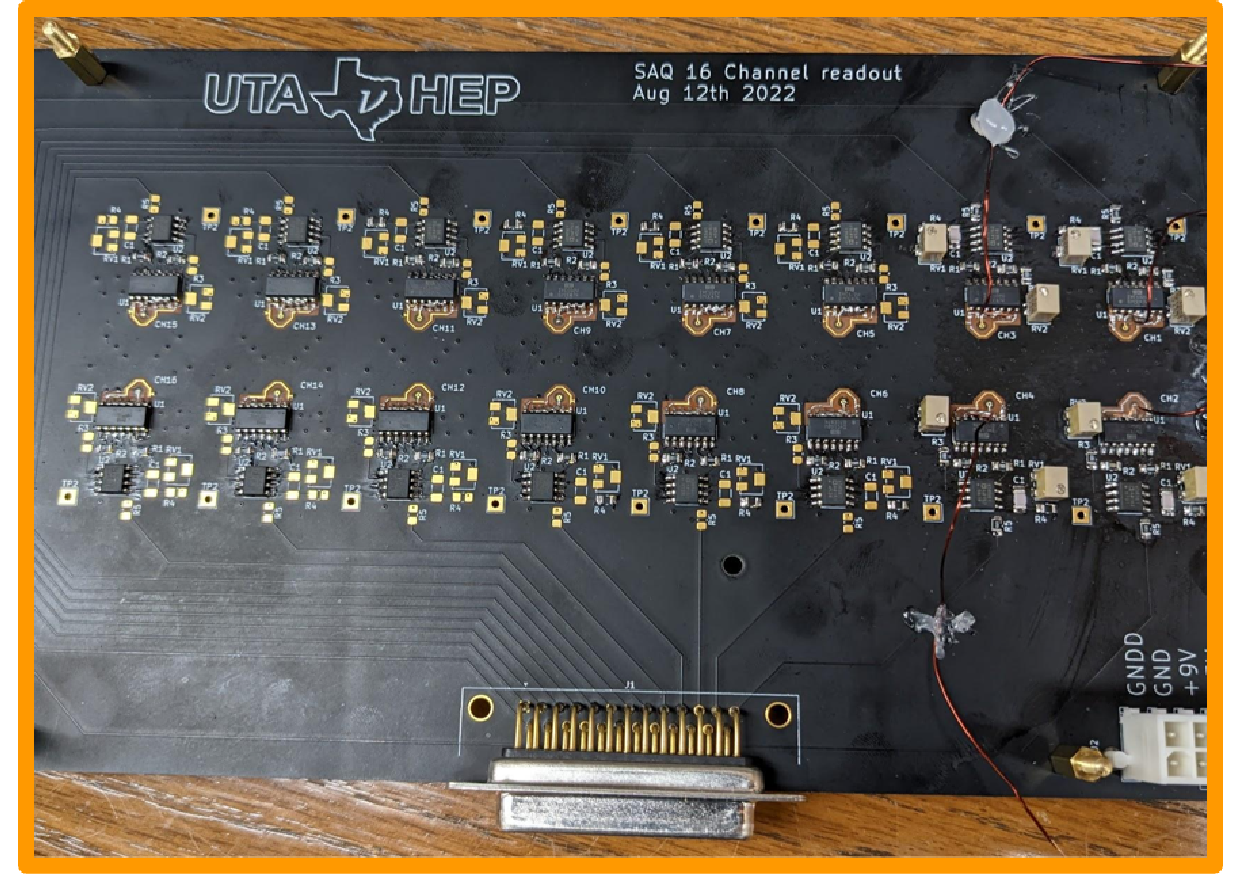
\includegraphics[width=\textwidth]{images/SAQ_16_ivc_readout_board.pdf}
\caption{The SAQ front-end board of 16 input IVC channels.
Each of the 16 channels are based on Figure~\ref{fig:saq_circuit_kicad}.
}
\label{fig:saq_readout_board}
\end{figure}


An example of resets produced from the comparator is shown in Figure~\ref{fig:saq_resets}.
The time difference between each reset shown is equivalent to the amount current accumulated at the IVC~(Equation~\ref{eq:irecon}).


\begin{figure}[]
\centering
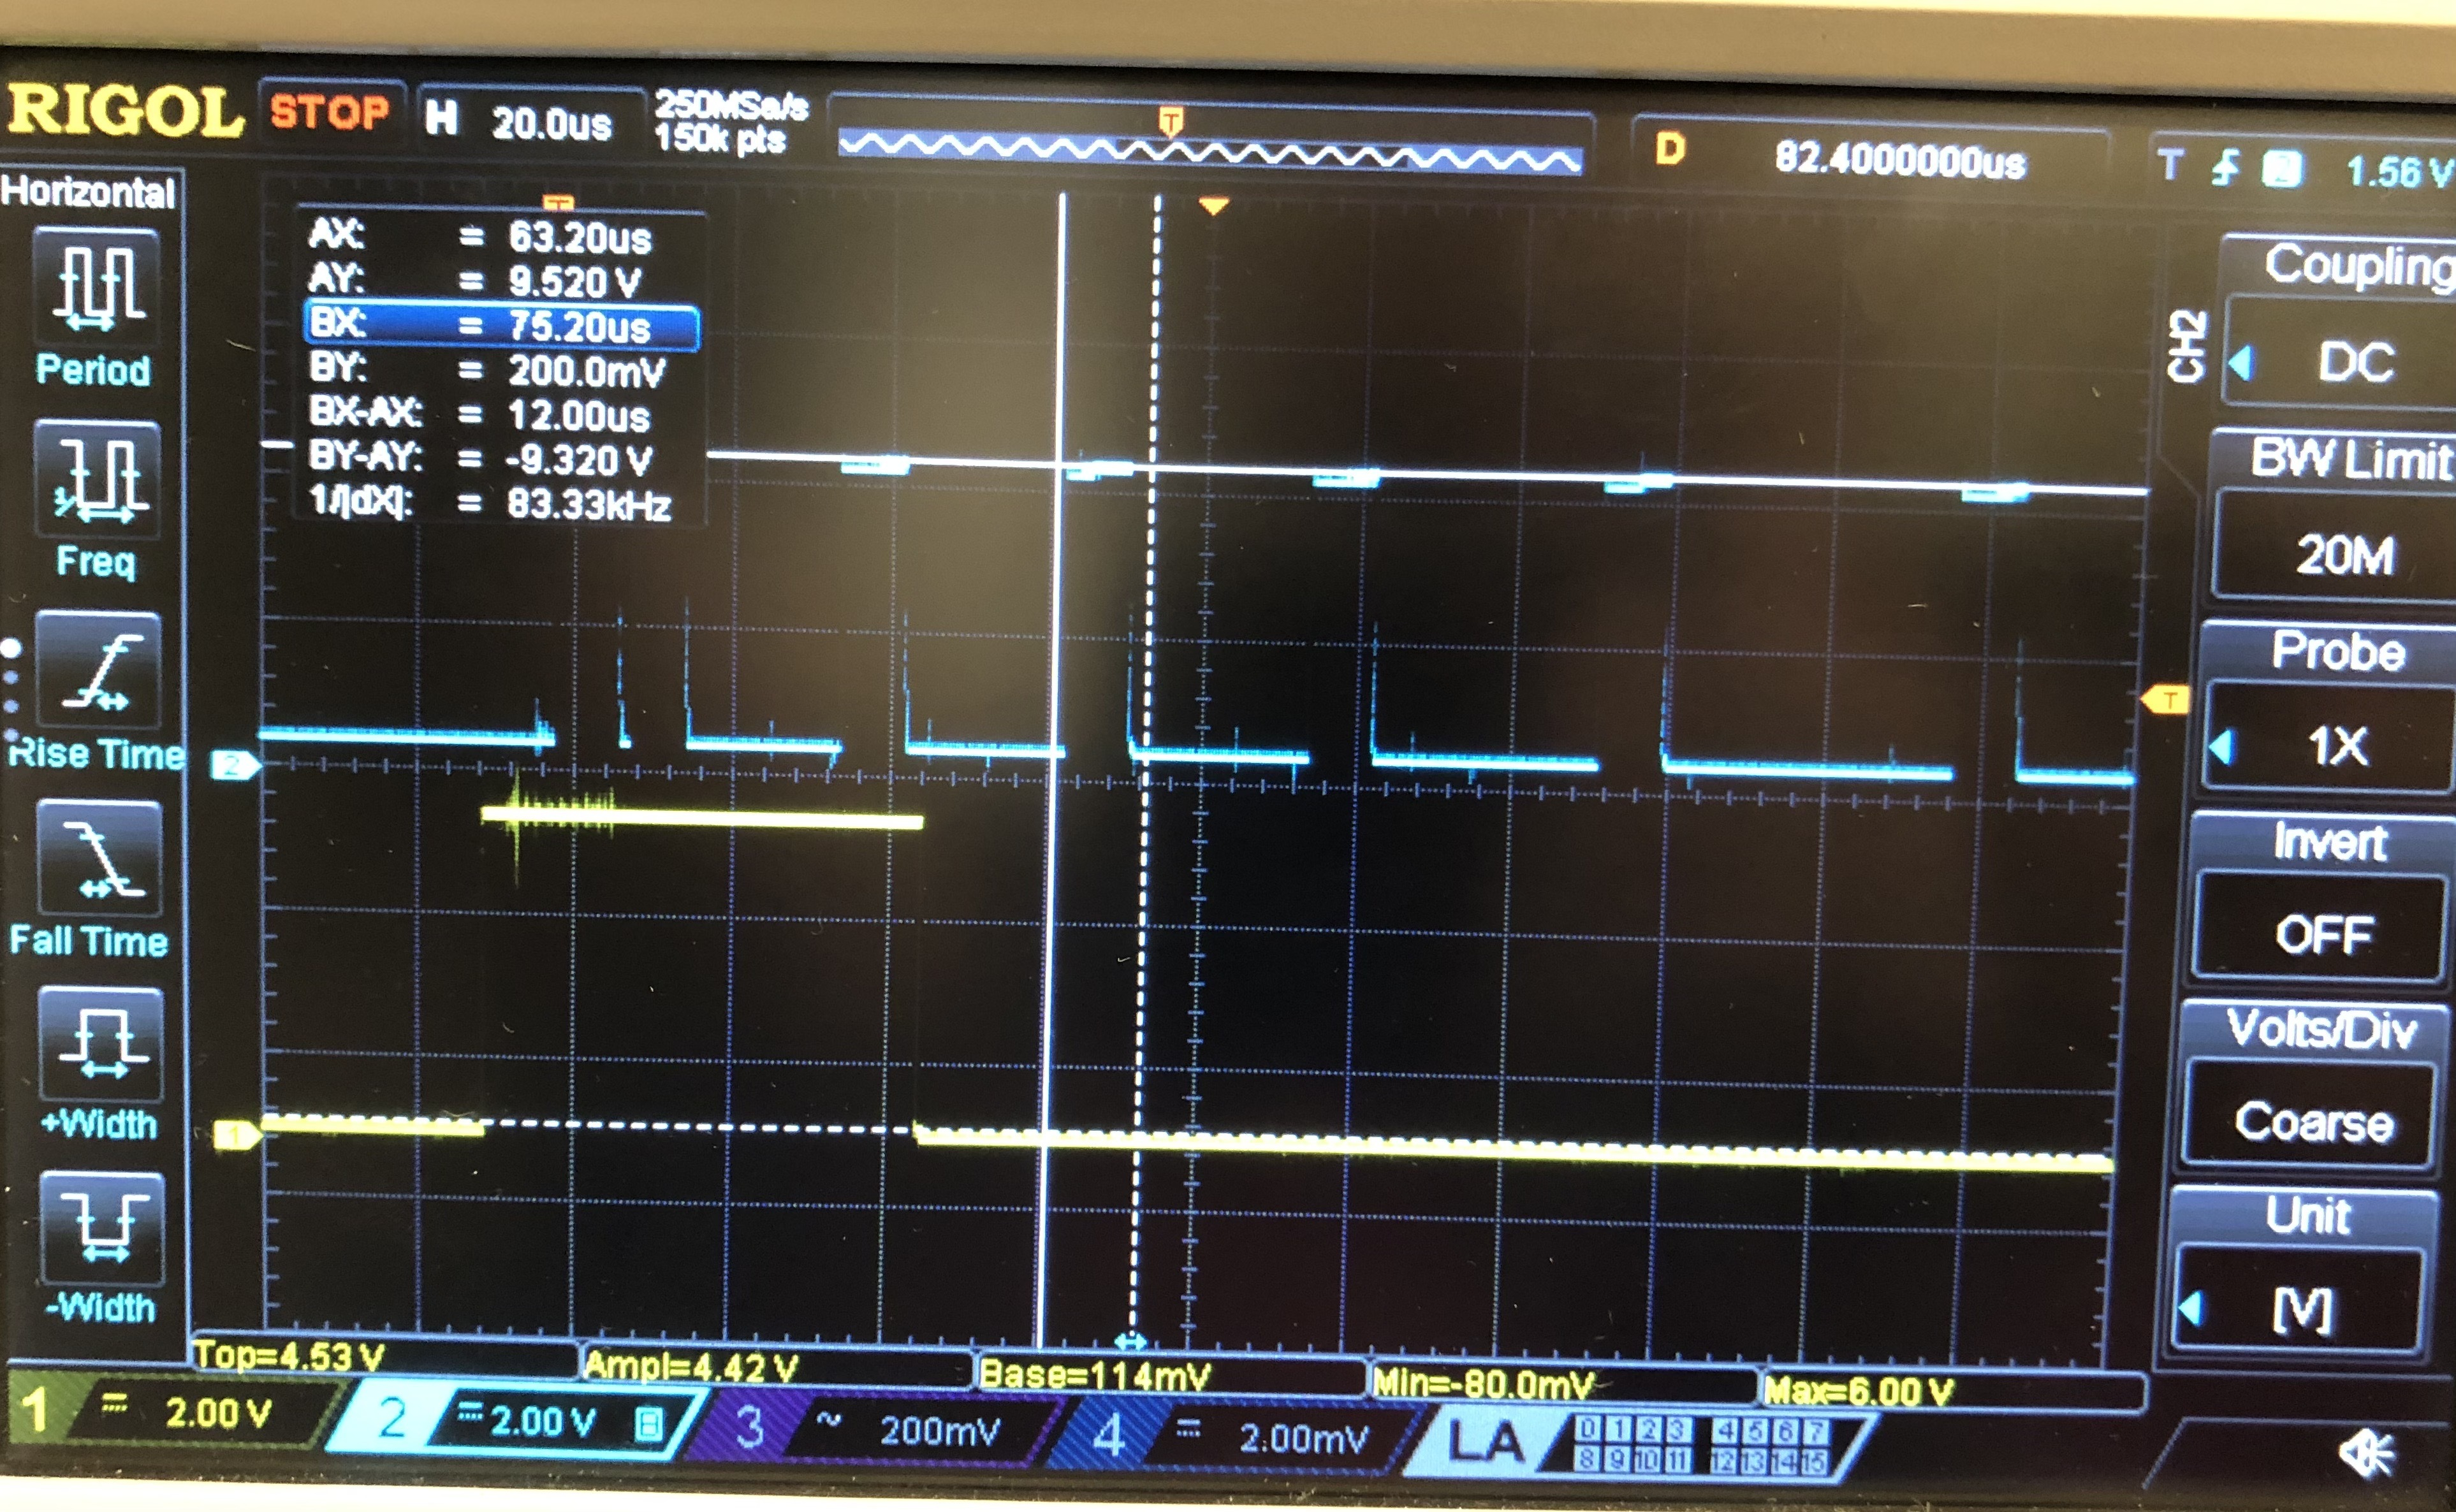
\includegraphics[width=\textwidth]{images/saq_reset_pulse_gem_thickBoard.jpg}
\caption{Waveform measurements of the trigger sent to the Xenon Flash lamp (yellow, bottom), and the reset pulse responses sent by the comparator.
Each reset corresponds to a build up of $\approx 10~\unit{pC}$ of charge stored up on the IVC capacitor.
Seen in the waveform is a decaying amount of charge buildup on the capacitor, which is reflected in the increasing time separation between successive resets.
}
\label{fig:saq_resets}
\end{figure}

\begin{figure}[]
\centering
\begin{subfigure}{.5\textwidth}
  \centering
  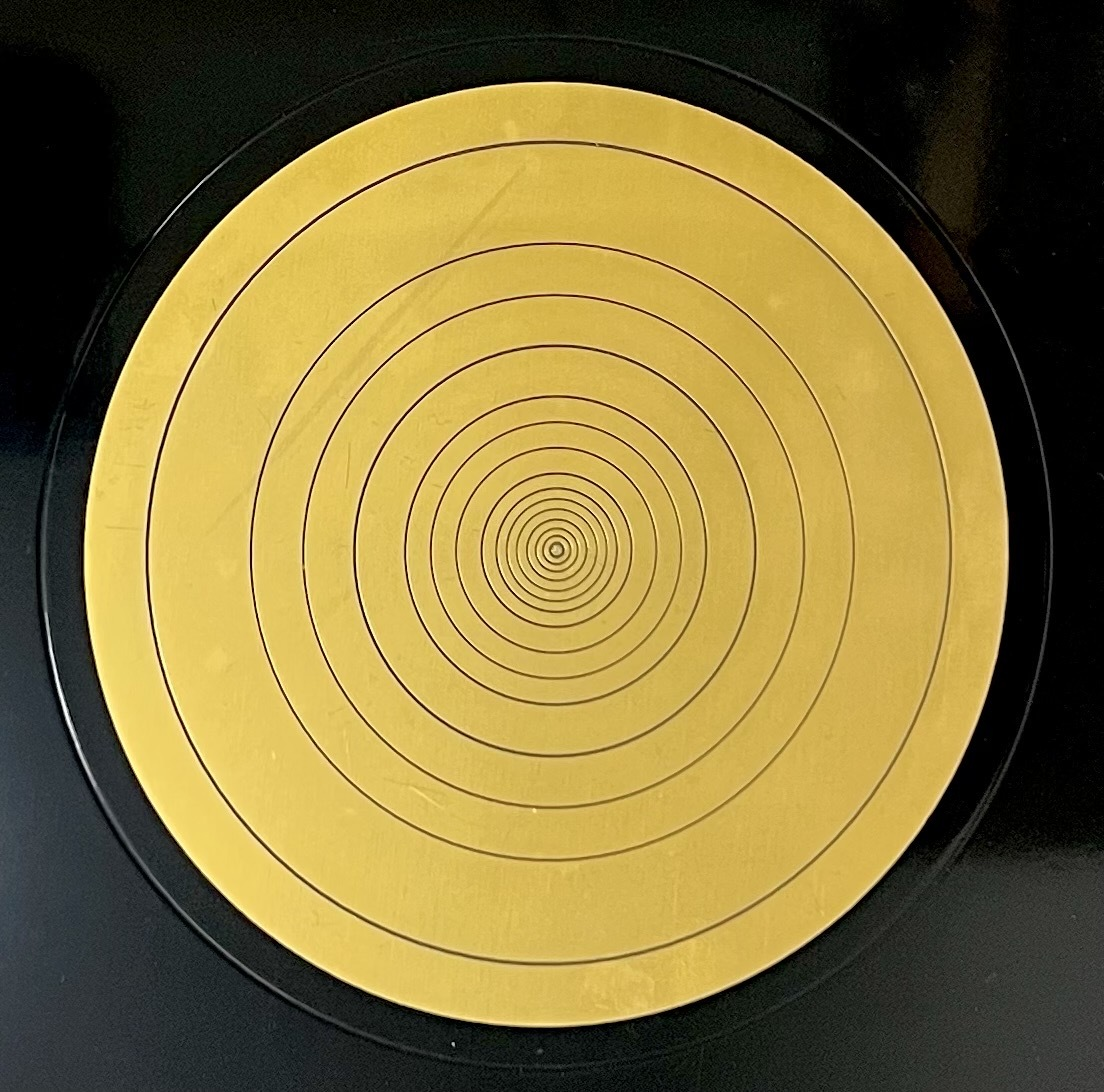
\includegraphics[width=\textwidth]{images/thick_board_example.jpg}
  \caption{}
\end{subfigure}%
\begin{subfigure}{.5\textwidth}
  \centering
  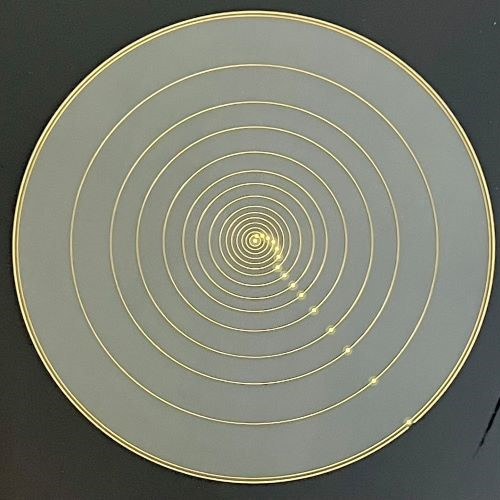
\includegraphics[width=\textwidth]{images/thin_trace_board_example.jpg}
  \caption{}
\end{subfigure}
\caption{Different Trace Boards used in the SAQ Experiment.}
\label{fig:trace_boards}
\end{figure}

\section{Data Acquisition}

All resets are recorded via a Zybo-Z7-20 Digilent FPGA prototype board, which uses an Artix Zynq based archticture.
The reference manual for the Zybo Z7 board used in SAQ can be found at~\citep{zybo_zy_reference}.

\begin{figure}[]
\centering
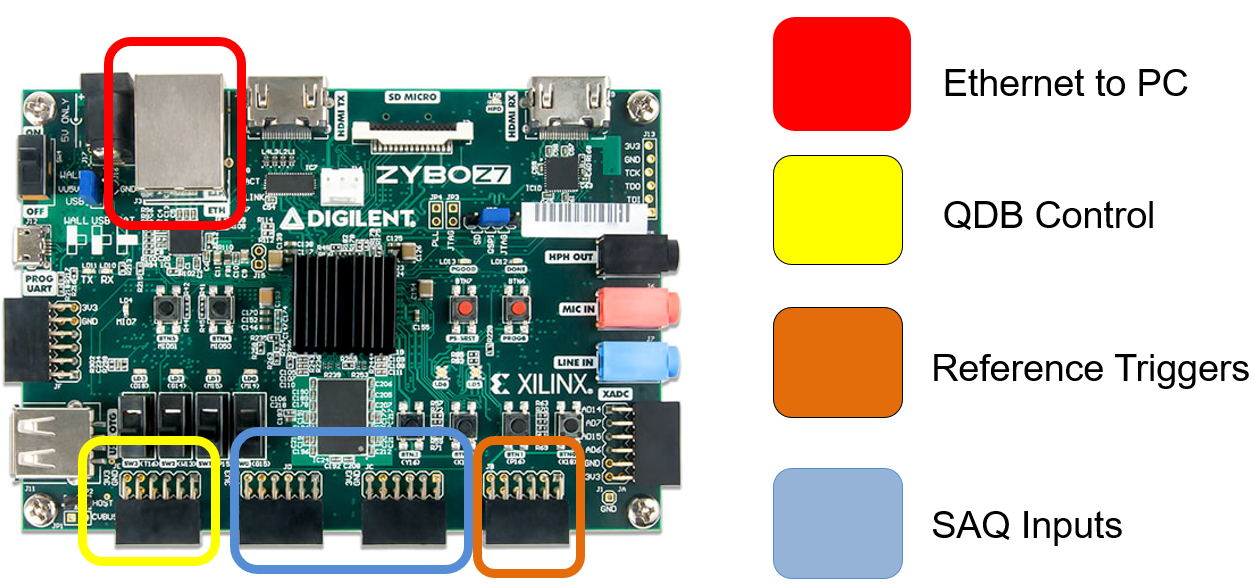
\includegraphics[width=\textwidth]{images/saq_zybo_io_summary.png}
\caption{An image of the data acquisition board from Digilent, Zybo Z7-20. 
This board was chosen for its multiple configurable input chanels, as well as the Zynq-based archiecture of the onboard FPGA.
Additionally, the use of the ethernet provides $1~\unit{GB}$ transfer speeds, which is more than sufficient for the application.
Packet data transfer rates have been verified with this readout at stable rates of 10~\unit{kHz}.
This board is also used to control the Q-Pix Digital Boards (QDB), discussed in Chapter~\ref{chap:qdb}.
}
\label{fig:saq_zybo}
\end{figure}

\begin{figure}[]
\centering
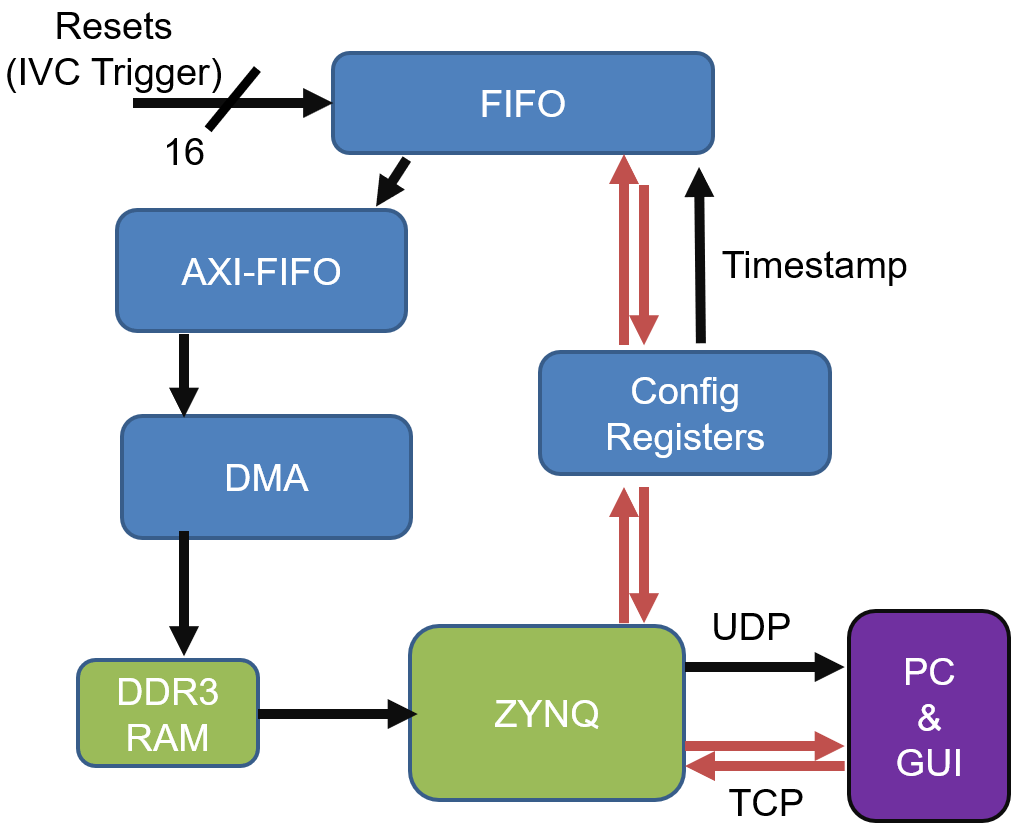
\includegraphics[width=\textwidth]{images/saq_daq_firmware_summary.png}
\caption{Firmware Description}
\label{fig:saq_firmware}
\end{figure}

\section{Pixel Calibration Procedure}

The Q-Pix readout is dependent on the integrator, which provides the basic datum of the reset time.
Therefore, a dominant source of noise are electrons which accumulate on the integrator which are not signal electrons.
There are two possible sources for these noise electrons: excess electrons produced from the target volume or leakage current due to transistor effects from the integrator circuit.
In this section we focus on the noise electrons due to the leakage current.

Leakage current arrises due to non-idyllic behavior of the integrator operational amplifier, where the voltage across the two input terminals is nonzero.
Measurements of this leakage current then are performed by measuring voltage difference across the terminals as well as directly using a pico-ammeter.

\subsection{Background Current in the GAr}

%% describe setup / filling of TPC here
The second source of noise electrons are produced from the target volume.
The target volume is an ultra pure Argon Gas at TODO militorr.
% 14 psi with argon (0.069 bar)
% And ~3mtorr of vacuum before that
In this case the excess electrons come from the nominal decay of Ar-39, which provide excess electrons from the natural $\beta$ decay, at a rate of $\approx 1~\unit{Bq}{Kg^{-1}}$

\section{Status and Discussion}


\begin{figure}[]
\centering
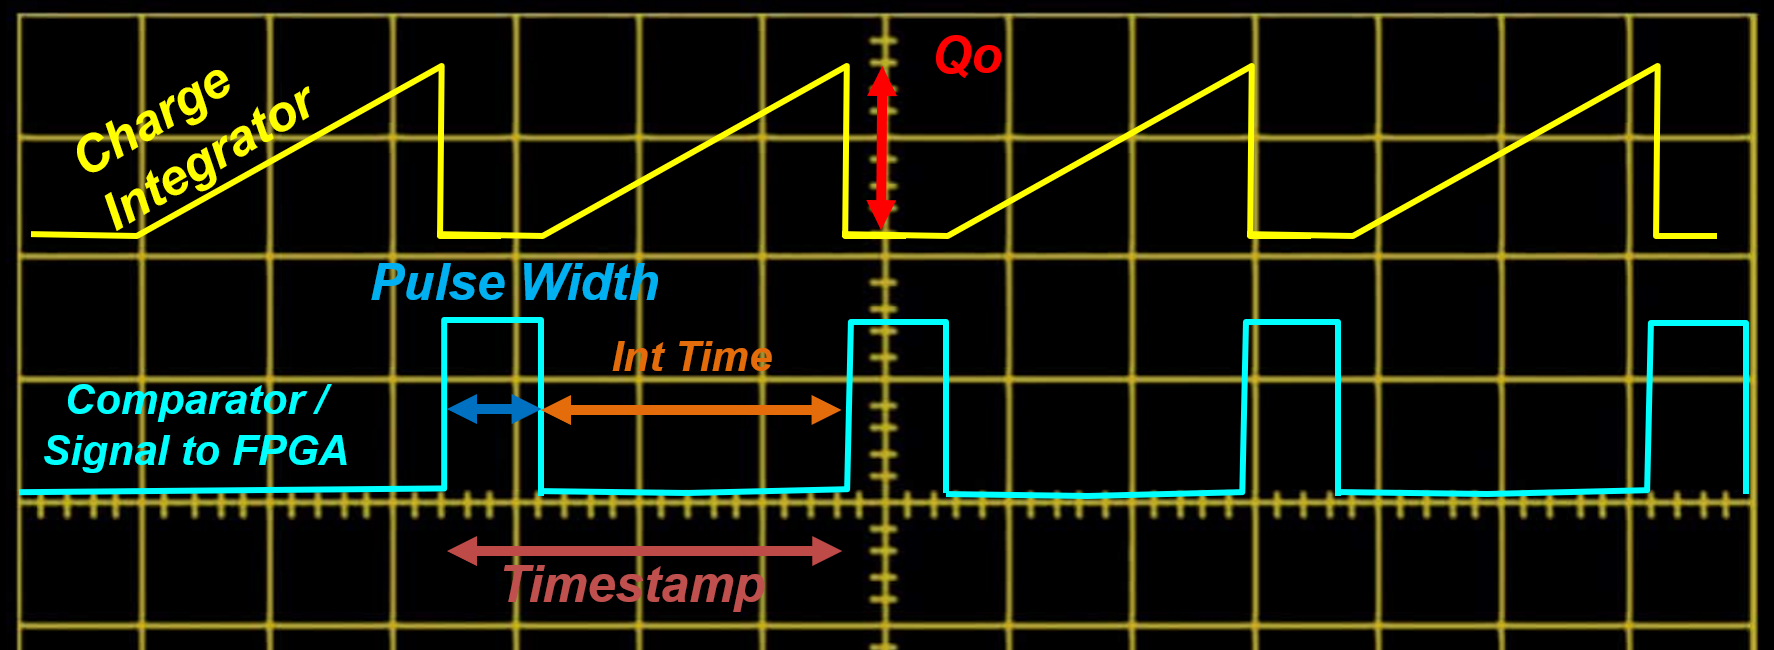
\includegraphics[width=\textwidth]{images/saq_example_reconstruction.png}
\caption{}
\label{fig:saq_reconstruction}
\end{figure}


\begin{figure}[]
\centering
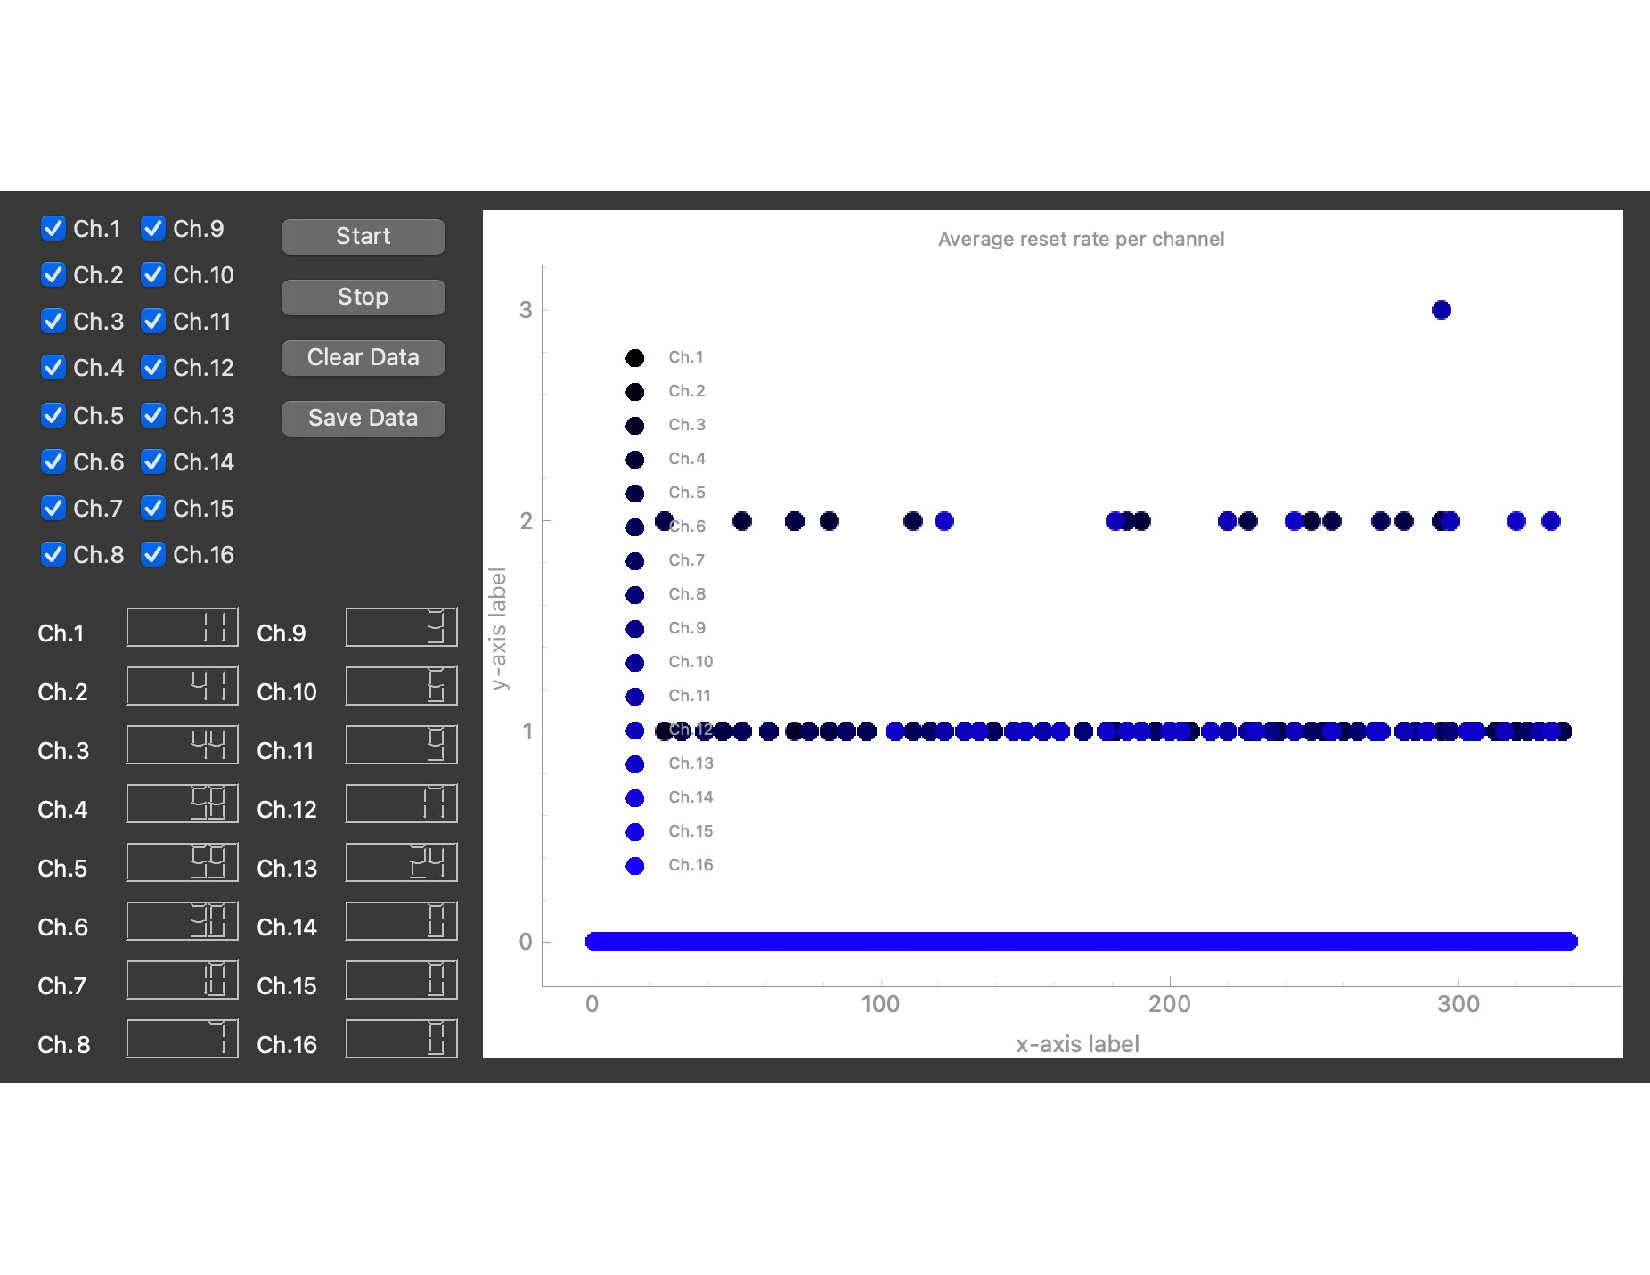
\includegraphics[width=\textwidth]{images/SAQ_gui_resets.pdf}
\caption{The SAQ GUI with real time plotting of incoming resets to the Zybo board.}
\label{fig:saq_gui}
\end{figure}


\subsection{Xenon Gas Lamp Measurements}

We use a Hamamatsu L13651 Xenon Gas Lamp to strike a gold foil.

\begin{figure}[]
\centering
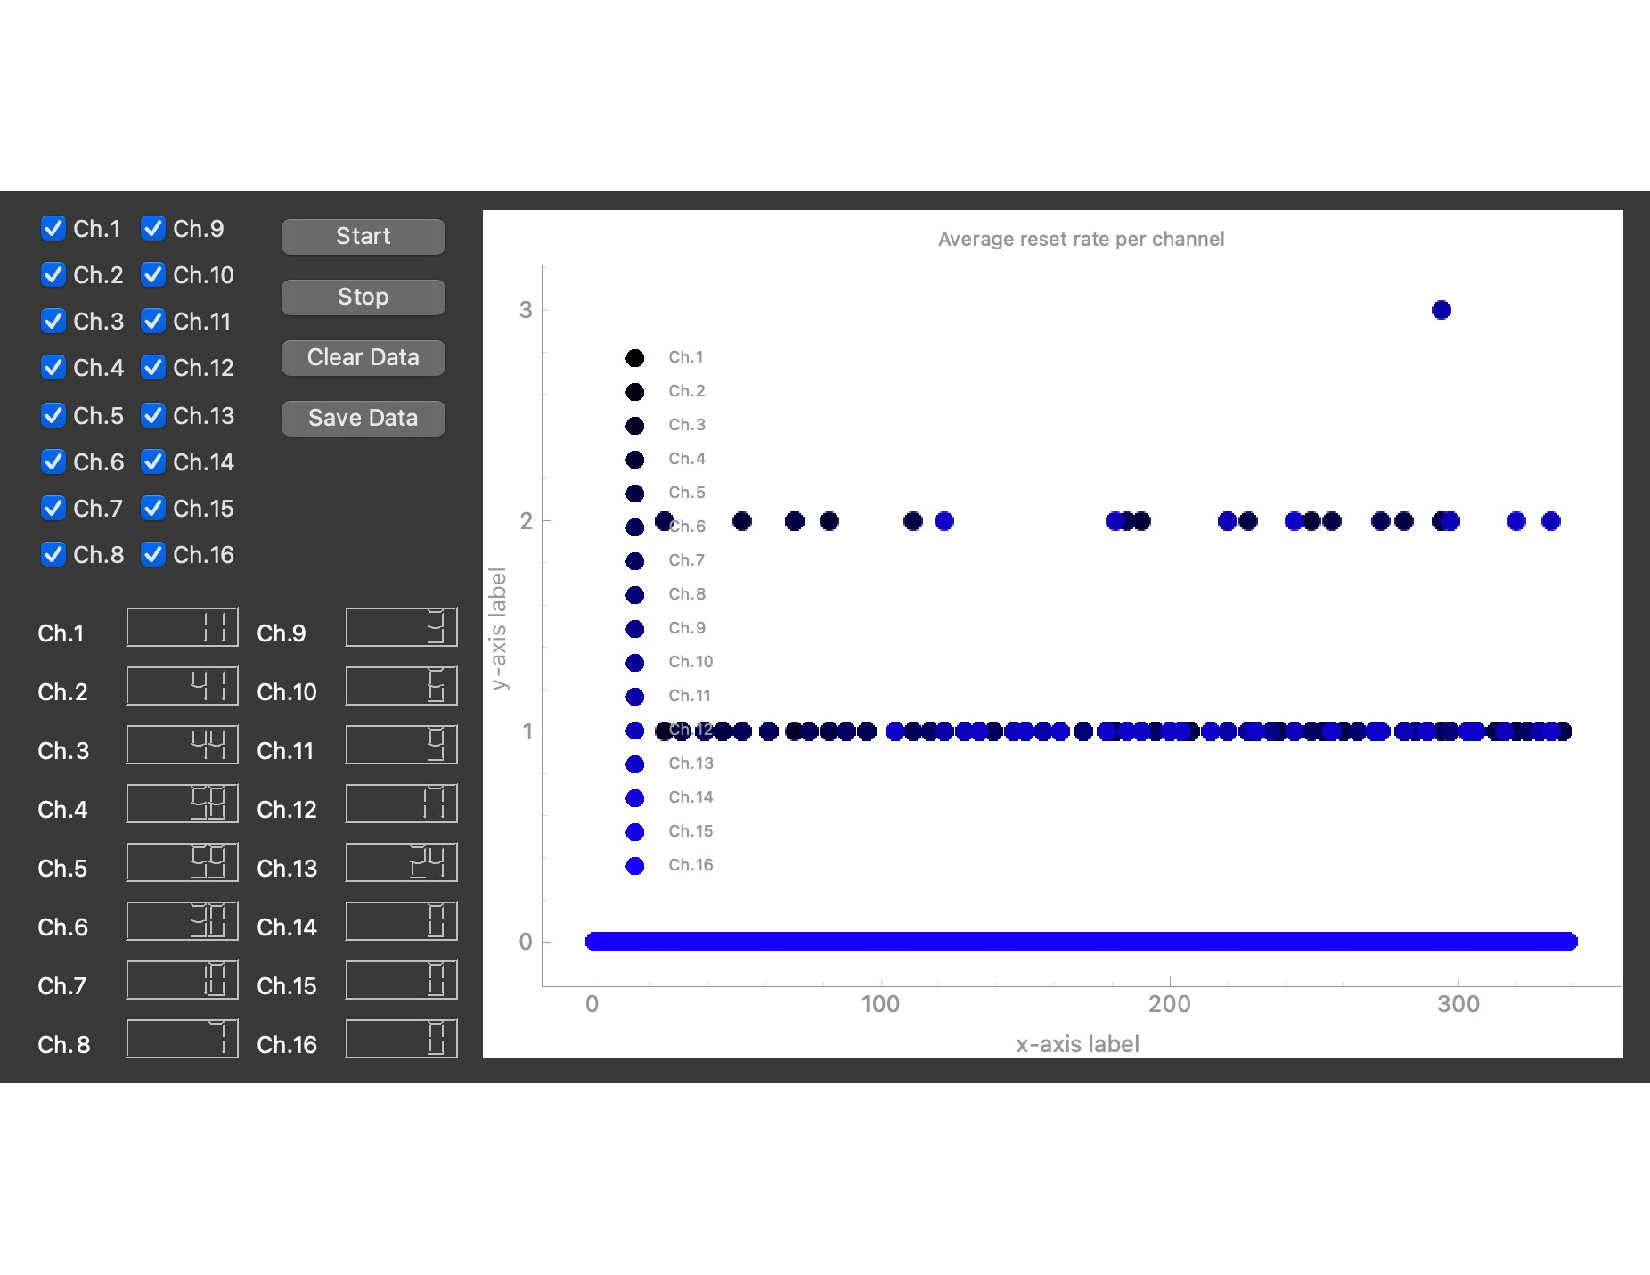
\includegraphics[width=\textwidth]{images/SAQ_gui_resets.pdf}
\caption{Drift Current Measurements to go here.}
\label{fig:saq_drift_gui}
\end{figure}

\subsection{State of Diffusion Measurements}

\begin{figure}[]
\centering
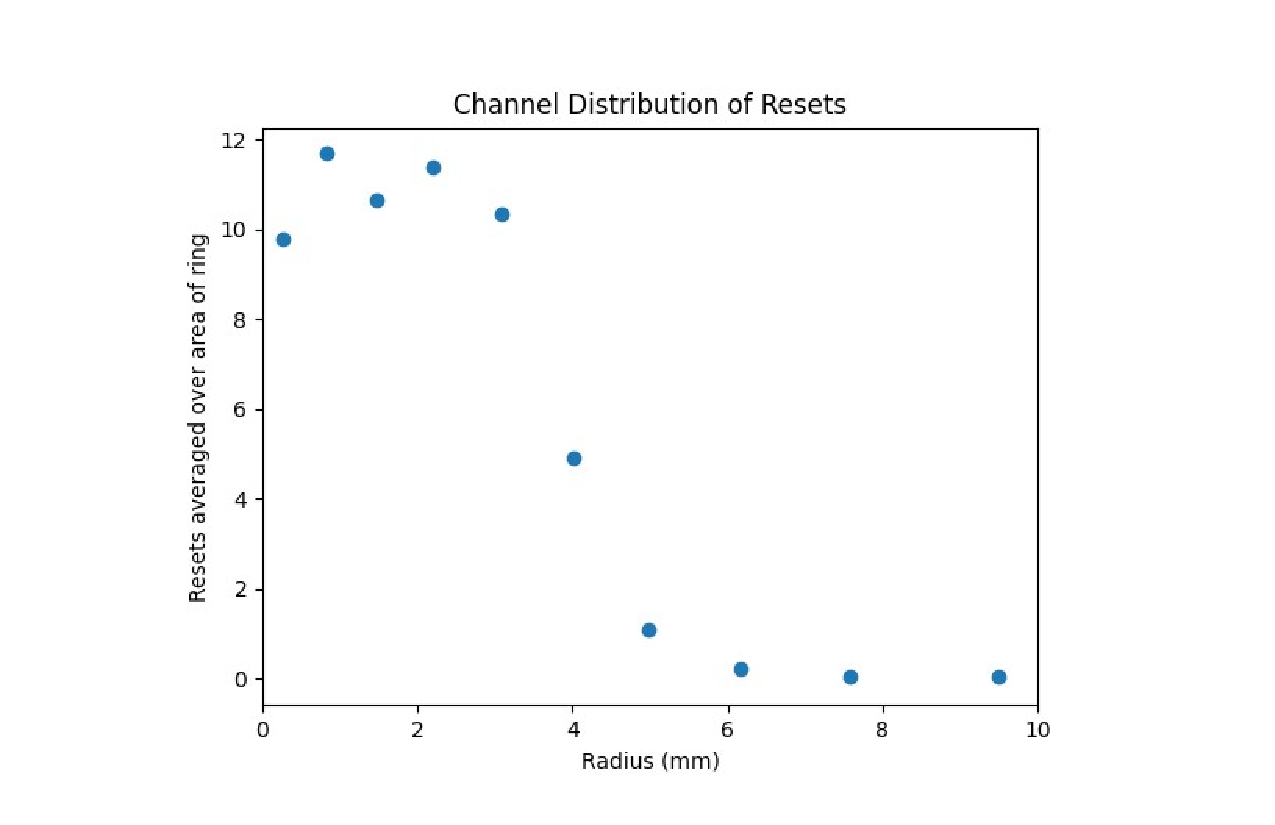
\includegraphics[width=\textwidth]{images/SAQ_first_diffusion_measurement.pdf}
\caption{First diffusion measurement in P-10 gas performed at Wellesy University.}
\label{fig:saq_first_diffusion_measurement}
\end{figure}

\subsection{Planned Measurements}

Measurements of Transverse and Longitudinal diffusion of electrons within electric fields of strength 500 V/cm have been performed before~\citep{lar_diffusion_measurement_LI2016160}.
